% vim: set spell spelllang=en tw=100 et sw=4 sts=4 :

\documentclass[a0paper]{tikzposter}

\usepackage{complexity}
\usepackage{wrapfig}
\usepackage{microtype}
\usepackage{gnuplot-lua-tikz}
\usepackage{amssymb}
\usepackage{amsmath}

\usepackage{lmodern}
\renewcommand*\familydefault{\sfdefault}
\usepackage[T1]{fontenc}

\title{Solving Hard Subgraph Problems in Parallel}
\author{Ciaran McCreesh and Patrick Prosser}
\institute{University of Glasgow, Glasgow, Scotland}
\titlegraphic{\includegraphics[keepaspectratio=true,scale=2.5]{UoG_keyline.pdf}}

\settitle{
    \begin{tikzpicture}
        \node (T) [inner sep=0pt] {\begin{minipage}{\linewidth}
                \color{titlefgcolor}
                {\bfseries \Huge \hspace{10mm}\@title \par}
                \vspace*{1em}
                {\Large {\bfseries \hspace{10mm}\@author}, \@institute}
        \end{minipage}};

        \node at (T.east) [anchor=center, inner sep=0pt, xshift=-8cm] {\@titlegraphic};
    \end{tikzpicture}
}

% University of Glasgow standard colours
\definecolor{uofguniversityblue}{rgb}{0, 0.219608, 0.396078}

\definecolor{uofgheather}{rgb}{0.356863, 0.32549, 0.490196}
\definecolor{uofgaquamarine}{rgb}{0.603922, 0.72549, 0.678431}
\definecolor{uofgslate}{rgb}{0.309804, 0.34902, 0.380392}
\definecolor{uofgrose}{rgb}{0.823529, 0.470588, 0.709804}
\definecolor{uofgmocha}{rgb}{0.709804, 0.564706, 0.47451}

\definecolor{uofglawn}{rgb}{0.517647, 0.741176, 0}
\definecolor{uofgcobalt}{rgb}{0, 0.615686, 0.92549}
\definecolor{uofgturquoise}{rgb}{0, 0.709804, 0.819608}
\definecolor{uofgsunshine}{rgb}{1.0, 0.862745, 0.211765}
\definecolor{uofgpumpkin}{rgb}{1.0, 0.72549, 0.282353}
\definecolor{uofgthistle}{rgb}{0.584314, 0.070588, 0.447059}
\definecolor{uofgpillarbox}{rgb}{0.701961, 0.047059, 0}
\definecolor{uofglavendar}{rgb}{0.356863, 0.301961, 0.580392}

\definecolor{uofgsandstone}{rgb}{0.321569, 0.278431, 0.231373}
\definecolor{uofgforest}{rgb}{0, 0.317647, 0.2}
\definecolor{uofgburgundy}{rgb}{0.490196, 0.133333, 0.223529}
\definecolor{uofgrust}{rgb}{0.603922, 0.227451, 0.023529}

\definecolorstyle{UofG}{
}{
    % Background Colors
    \colorlet{backgroundcolor}{uofgsandstone!80!white}
    \colorlet{framecolor}{black}
    % Title Colors
    \colorlet{titlefgcolor}{white}
    \colorlet{titlebgcolor}{uofguniversityblue}
    % Block Colors
    \colorlet{blocktitlebgcolor}{white}
    \colorlet{blocktitlefgcolor}{uofguniversityblue}
    \colorlet{blockbodybgcolor}{white}
    \colorlet{blockbodyfgcolor}{black}
    % Innerblock Colors
    \colorlet{innerblocktitlebgcolor}{uofguniversityblue}
    \colorlet{innerblocktitlefgcolor}{black}
    \colorlet{innerblockbodybgcolor}{uofgsandstone}
    \colorlet{innerblockbodyfgcolor}{black}
    % Note colors
    \colorlet{notefgcolor}{black}
    \colorlet{notebgcolor}{uofgrust}
    \colorlet{noteframecolor}{red}
}

\usetheme{Autumn}
\usecolorstyle{UofG}

\tikzposterlatexaffectionproofoff

\useblockstyle[bodyverticalshift=-1cm, roundedcorners=1]{Default}

\renewcommand{\Huge}{\fontsize{77.2}{96}\selectfont}

% Styles for drawings

\tikzset{edge/.style={line width=3pt, color=uofgsandstone}}
\tikzset{ledge/.style={line width=3pt, color=uofgsandstone!40!white}}

\setlength\intextsep{0pt}

\begin{document}
\maketitle

{
    \colorlet{blockbodybgcolor}{uofgcobalt}
    \colorlet{blocktitlebgcolor}{uofgcobalt}
    \block[bodyverticalshift=0cm, bodyinnersep=3mm]{}{
        \centering\begin{minipage}{0.94\textwidth}
            \textbf{Graphs} allow us to model complex and dynamic relationships, and by
            \textbf{finding subgraphs} we can identify interesting properties and structures. In
            general, subgraph problems are \NP-hard (very informally, adding just one extra
            vertex doubles the difficulty), but practical algorithms can avoid hitting the
            exponential worst-case for many real-world inputs. We investigate how we can
            \textbf{exploit the parallelism} present in multi-core processors to \textbf{speed up} solving
            hard subgraph problems, or to allow us to tackle \textbf{larger or more complicated
            problems} in the time we have.
        \end{minipage}
    }
}

\begin{columns}
\column{0.5}

\block{Clique (Finding Groups of Mutual Friends)}{
\begin{wrapfigure}[8]{r}{0.4\linewidth}
    \vspace*{0.5cm}
    \begin{center}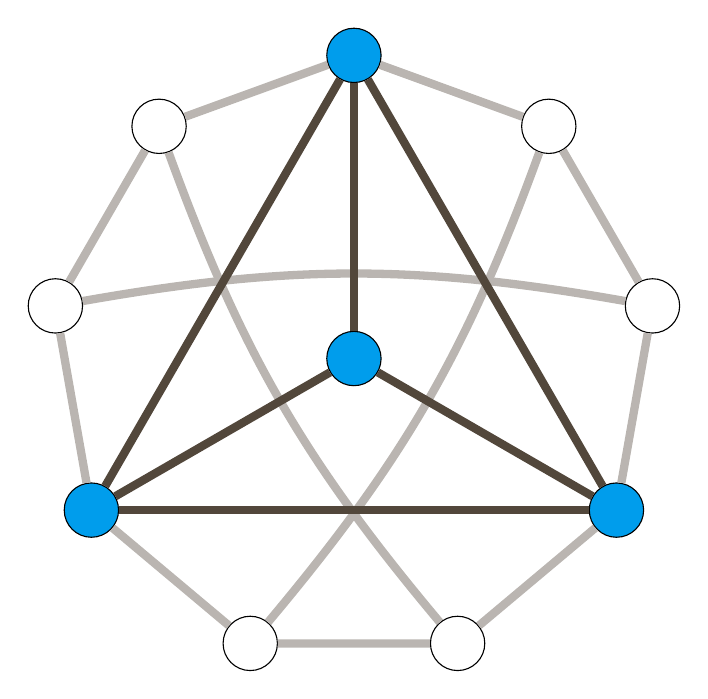
\begin{tikzpicture}[scale=1.75]%{{{
        \newcount \c
        \foreach \n in {1, ..., 9}{
            \c=\n \advance\c by -1 \multiply\c by -360 \divide\c by 9 \advance\c by 290.0
            \ifthenelse{\n = 3 \OR \n = 6 \OR \n = 9}{
                \node[draw, circle, fill=uofgcobalt, inner sep=5pt, font=\bfseries] (N\n) at (\the\c:2.2) {\vphantom{0}};
            }{
                \node[draw, circle, fill=white, inner sep=5pt, font=\bfseries] (N\n) at (\the\c:2.2) {\vphantom{0}};
            }
        }
        \node[draw, circle, fill=uofgcobalt, inner sep=5pt, font=\bfseries] (N10) at (0, 0) {\vphantom{0}};

        \draw [ledge] (N1) -- (N2);
        \draw [ledge] (N2) -- (N3);
        \draw [ledge] (N3) -- (N4);
        \draw [ledge] (N4) -- (N5);
        \draw [ledge] (N5) -- (N6);
        \draw [ledge] (N6) -- (N7);
        \draw [ledge] (N7) -- (N8);
        \draw [ledge] (N8) -- (N9);
        \draw [ledge] (N9) -- (N1);

        \draw [ledge] (N4) to [out=10, in=170] (N8);
        \draw [ledge] (N2) to [out=50, in=250] (N7);
        \draw [ledge] (N5) to [out=290, in=130] (N1);

        \draw [edge] (N3) -- (N10);
        \draw [edge] (N6) -- (N10);
        \draw [edge] (N9) -- (N10);
        \draw [edge] (N6) -- (N3);
        \draw [edge] (N9) -- (N3);
        \draw [edge] (N6) -- (N9);
    \end{tikzpicture}\end{center}
\end{wrapfigure}

    A \textbf{clique} can be thought of as a group of people, where everyone in the group knows
    everyone else in the group.  Finding cliques lets us select \textbf{as much of a resource as
    possible}, respecting compatibility rules. Clique-finding algorithms have been used for
        verifying electronic circuits, to improve the reliability of communications and networking
        protocols, for social media analysis, for targeted advertising, and for controlling flying
        robots.
    }

\block{Subgraph Isomorphism (Finding Patterns)}{
\begin{wrapfigure}[11]{r}{0.4\linewidth}
    \vspace*{0.5cm}
    \begin{center}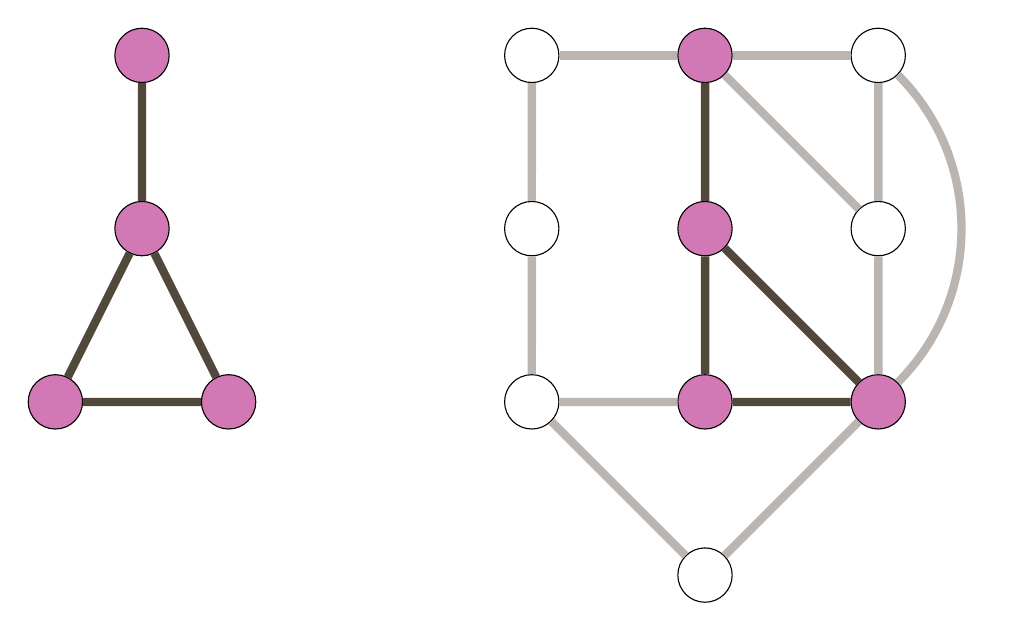
\begin{tikzpicture}[scale=1.1]%{{{
        \node[draw, circle, fill=uofgrose, inner sep=5pt, font=\bfseries] (Na) at (1,  0)
        {\vphantom{0}};
        \node[draw, circle, fill=uofgrose, inner sep=5pt, font=\bfseries] (Nb) at (1, -2)
        {\vphantom{0}};
        \node[draw, circle, fill=uofgrose, inner sep=5pt, font=\bfseries] (Nc) at (0, -4)
        {\vphantom{0}};
        \node[draw, circle, fill=uofgrose, inner sep=5pt, font=\bfseries] (Nd) at (2, -4)
        {\vphantom{0}};

        \draw [edge] (Na) -- (Nb);
        \draw [edge] (Nb) -- (Nc);
        \draw [edge] (Nc) -- (Nd);
        \draw [edge] (Nb) -- (Nd);

        \node[draw, circle, fill=uofgrose, inner sep=5pt, font=\bfseries] (N1) at (7.5,  0) {\vphantom{0}};
        \node[draw, circle, fill=white, inner sep=5pt, font=\bfseries] (N2) at (9.5,  0) {\vphantom{0}};
        \node[draw, circle, fill=uofgrose, inner sep=5pt, font=\bfseries] (N3) at (7.5, -2) {\vphantom{0}};
        \node[draw, circle, fill=white, inner sep=5pt, font=\bfseries] (N4) at (9.5, -2) {\vphantom{0}};
        \node[draw, circle, fill=uofgrose, inner sep=5pt, font=\bfseries] (N5) at (7.5, -4) {\vphantom{0}};
        \node[draw, circle, fill=uofgrose, inner sep=5pt, font=\bfseries] (N6) at (9.5, -4) {\vphantom{0}};
        \node[draw, circle, fill=white, inner sep=5pt, font=\bfseries] (N7) at (5.5,  0) {\vphantom{0}};
        \node[draw, circle, fill=white, inner sep=5pt, font=\bfseries] (N8) at (5.5, -2) {\vphantom{0}};
        \node[draw, circle, fill=white, inner sep=5pt, font=\bfseries] (N9) at (5.5, -4) {\vphantom{0}};
        \node[draw, circle, fill=white, inner sep=5pt, font=\bfseries] (N10) at (7.5, -6) {\vphantom{0}};

        \draw [ledge] (N1) -- (N2);
        \draw [edge] (N1) -- (N3);
        \draw [ledge] (N1) -- (N4);
        \draw [ledge] (N2) -- (N4);
        \draw [edge] (N3) -- (N5);
        \draw [edge] (N3) -- (N6);
        \draw [ledge] (N4) -- (N6);
        \draw [edge] (N5) -- (N6);
        \draw [ledge] (N2) to [in=45, out=315] (N6);
        \draw [ledge] (N1) -- (N7);
        \draw [ledge] (N5) -- (N9);
        \draw [ledge] (N7) -- (N8);
        \draw [ledge] (N8) -- (N9);
        \draw [ledge] (N6) -- (N10);
        \draw [ledge] (N9) -- (N10);
    \end{tikzpicture}\end{center}
\end{wrapfigure}

    Many real-world phenomena, such as social networks, transport routes, financial transactions,
    and chemical molecules, can be described using graphs. We may wish to \textbf{find interesting
    structures} inside these graphs. The subgraph isomorphism problem is to find a small ``pattern''
    graph in a big ``target'' graph. This is useful in drug design, in fraud detection, in fault
    diagnosis, and in source code analysis.
}

\block{Maximum Common Subgraph (Comparing Graphs)}{
    We can also \textbf{compare two graphs}. We do this via the maximum common subgraph problem,
    which is to find the largest subgraph common to two bigger graphs. This is useful directly in
    computer vision, database searches, and biochemistry, and it also lets us find
    \textbf{approximate solutions} when a subgraph isomorphism query fails.

    \vspace*{1cm}

    \begin{center}\begin{tikzpicture}[scale=1.1]%{{{
        \begin{scope}[]
            \node[draw, circle, fill=uofgpumpkin, inner sep=5pt, font=\bfseries] (M1) at (90:2) {\vphantom{0}};
            \node[draw, circle, fill=uofgpumpkin, inner sep=5pt, font=\bfseries] (M2) at (150:2) {\vphantom{0}};
            \node[draw, circle, fill=uofgpumpkin, inner sep=5pt, font=\bfseries] (M3) at (30:2) {\vphantom{0}};
            \node[draw, circle, fill=uofgpumpkin, inner sep=5pt, font=\bfseries] (M4) at (210:2) {\vphantom{0}};
            \node[draw, circle, fill=uofgpumpkin, inner sep=5pt, font=\bfseries] (M5) at (330:2) {\vphantom{0}};
            \node[draw, circle, fill=white, inner sep=5pt, font=\bfseries] (M6) at (270:2) {\vphantom{0}};
            \node[draw, circle, fill=uofgpumpkin, inner sep=5pt, font=\bfseries] (M7) at ($(210:2) + (M6)$) {\vphantom{0}};
            \node[draw, circle, fill=uofgpumpkin, inner sep=5pt, font=\bfseries] (M8) at ($(330:2) + (M6)$) {\vphantom{0}};
            \node[draw, circle, fill=uofgpumpkin, inner sep=5pt, font=\bfseries] (M9) at ($(270:2) + (M6)$) {\vphantom{0}};

            \draw [edge] (M1) -- (M2);
            \draw [edge] (M2) -- (M4);
            \draw [edge] (M3) -- (M5);
            \draw [ledge] (M4) -- (M6);
            \draw [ledge] (M5) -- (M6);
            \draw [edge] (M3) -- (M1);
            \draw [ledge] (M6) -- (M7);
            \draw [ledge] (M6) -- (M8);
            \draw [ledge] (M6) -- (M9);
            \draw [edge] (M7) -- (M9);
            \draw [edge] (M8) -- (M9);
        \end{scope}

        \begin{scope}[xshift=7cm]
            \node[draw, circle, fill=uofgpumpkin, inner sep=5pt, font=\bfseries] (M1) at (90:2) {\vphantom{0}};
            \node[draw, circle, fill=uofgpumpkin, inner sep=5pt, font=\bfseries] (M2) at (150:2) {\vphantom{0}};
            \node[draw, circle, fill=uofgpumpkin, inner sep=5pt, font=\bfseries] (M3) at (30:2) {\vphantom{0}};
            \node[draw, circle, fill=uofgpumpkin, inner sep=5pt, font=\bfseries] (M4) at (210:2) {\vphantom{0}};
            \node[draw, circle, fill=uofgpumpkin, inner sep=5pt, font=\bfseries] (M5) at (330:2) {\vphantom{0}};
            \node[draw, circle, fill=white, inner sep=5pt, font=\bfseries] (M6) at (270:2) {\vphantom{0}};
            \node[draw, circle, fill=uofgpumpkin, inner sep=5pt, font=\bfseries] (M7) at ($(210:2) + (M6)$) {\vphantom{0}};
            \node[draw, circle, fill=uofgpumpkin, inner sep=5pt, font=\bfseries] (M8) at ($(270:2) + (M6)$) {\vphantom{0}};
            \node[draw, circle, fill=uofgpumpkin, inner sep=5pt, font=\bfseries] (M9) at ($(330:2) + (M8)$) {\vphantom{0}};

            \draw [edge] (M1) -- (M2);
            \draw [edge] (M2) -- (M4);
            \draw [edge] (M3) -- (M5);
            \draw [ledge] (M4) -- (M6);
            \draw [ledge] (M5) -- (M6);
            \draw [edge] (M3) -- (M1);
            \draw [ledge] (M6) -- (M7);
            \draw [edge] (M7) -- (M8);
            \draw [edge] (M8) -- (M9);
        \end{scope}

        \begin{scope}[xshift=17cm]
            \node[draw, circle, fill=uofgcobalt, inner sep=5pt, font=\bfseries] (M1) at (90:2) {\vphantom{0}};
            \node[draw, circle, fill=uofgcobalt, inner sep=5pt, font=\bfseries] (M2) at (150:2) {\vphantom{0}};
            \node[draw, circle, fill=uofgcobalt, inner sep=5pt, font=\bfseries] (M3) at (30:2) {\vphantom{0}};
            \node[draw, circle, fill=uofgcobalt, inner sep=5pt, font=\bfseries] (M4) at (210:2) {\vphantom{0}};
            \node[draw, circle, fill=uofgcobalt, inner sep=5pt, font=\bfseries] (M5) at (330:2) {\vphantom{0}};
            \node[draw, circle, fill=uofgcobalt, inner sep=5pt, font=\bfseries] (M6) at (270:2) {\vphantom{0}};
            \node[draw, circle, fill=white, inner sep=5pt, font=\bfseries] (M7) at ($(210:2) + (M6)$) {\vphantom{0}};
            \node[draw, circle, fill=uofgcobalt, inner sep=5pt, font=\bfseries] (M8) at ($(330:2) + (M6)$) {\vphantom{0}};
            \node[draw, circle, fill=white, inner sep=5pt, font=\bfseries] (M9) at ($(270:2) + (M6)$) {\vphantom{0}};

            \draw [edge] (M1) -- (M2);
            \draw [edge] (M2) -- (M4);
            \draw [edge] (M3) -- (M5);
            \draw [edge] (M4) -- (M6);
            \draw [edge] (M5) -- (M6);
            \draw [edge] (M3) -- (M1);
            \draw [ledge] (M6) -- (M7);
            \draw [edge] (M6) -- (M8);
            \draw [ledge] (M6) -- (M9);
            \draw [ledge] (M7) -- (M9);
            \draw [ledge] (M8) -- (M9);
        \end{scope}

        \begin{scope}[xshift=24cm]
            \node[draw, circle, fill=uofgcobalt, inner sep=5pt, font=\bfseries] (M1) at (90:2) {\vphantom{0}};
            \node[draw, circle, fill=uofgcobalt, inner sep=5pt, font=\bfseries] (M2) at (150:2) {\vphantom{0}};
            \node[draw, circle, fill=uofgcobalt, inner sep=5pt, font=\bfseries] (M3) at (30:2) {\vphantom{0}};
            \node[draw, circle, fill=uofgcobalt, inner sep=5pt, font=\bfseries] (M4) at (210:2) {\vphantom{0}};
            \node[draw, circle, fill=uofgcobalt, inner sep=5pt, font=\bfseries] (M5) at (330:2) {\vphantom{0}};
            \node[draw, circle, fill=uofgcobalt, inner sep=5pt, font=\bfseries] (M6) at (270:2) {\vphantom{0}};
            \node[draw, circle, fill=uofgcobalt, inner sep=5pt, font=\bfseries] (M7) at ($(210:2) + (M6)$) {\vphantom{0}};
            \node[draw, circle, fill=white, inner sep=5pt, font=\bfseries] (M8) at ($(270:2) + (M6)$) {\vphantom{0}};
            \node[draw, circle, fill=white, inner sep=5pt, font=\bfseries] (M9) at ($(330:2) + (M8)$) {\vphantom{0}};

            \draw [edge] (M1) -- (M2);
            \draw [edge] (M2) -- (M4);
            \draw [edge] (M3) -- (M5);
            \draw [edge] (M4) -- (M6);
            \draw [edge] (M5) -- (M6);
            \draw [edge] (M3) -- (M1);
            \draw [edge] (M6) -- (M7);
            \draw [ledge] (M7) -- (M8);
            \draw [ledge] (M8) -- (M9);
        \end{scope}
    \end{tikzpicture}\end{center}

    \vspace*{0.8cm}

    An interesting variation of the problem requires the common subgraph to be \textbf{connected},
    as shown on the right---this can give more sensible results when comparing molecules.
}

\column{0.5}

\block{Parallel Search: Irregularity, Heuristics, and Diversity}{
    Practical algorithms for these problems combine \textbf{inference} (like you do when crossing
    out numbers when solving a Sudoku puzzle) and \textbf{backtracking search} (when we have to
    guess).  Even with the best algorithms and implementations, though, solving hard graph problems
    can take longer than we would like. We might hope that we could use the multiple cores provided
    by modern processors to make our programs \textbf{run faster}, or at least to \textbf{solve
    larger or harder problems} in the time we have.

    We may view the recursive calls made by a backtracking search algorithm as forming a tree. This
    lets us \textbf{speculatively evaluate many sub-trees simultaneously} using parallel hardware.
    However, static decomposition often leads to \textbf{poor work balance}:

    \vspace{1cm}

    \begin{center}
    \begin{tikzpicture}[scale=2.5]%{{{
        \coordinate (R);

        \coordinate (N) at (R);

        \coordinate (N1) at ($(N) + (-4, -0.75)$);
        \coordinate (N2) at ($(N) + ( 0, -0.75)$);
        \coordinate (N3) at ($(N) + ( 4, -0.75)$);

        \foreach \na in {1, ..., 3}{
            \coordinate (N\na 1) at ($(N\na) + (-1.25, -1)$);
            \coordinate (N\na 2) at ($(N\na) + ( 0,    -1)$);
            \coordinate (N\na 3) at ($(N\na) + ( 1.25, -1)$);

            \foreach \nb in {1, ..., 3}{
                \coordinate (N\na\nb t1) at ($(N\na\nb) + (-0.45, -1)$);
                \coordinate (N\na\nb t2) at ($(N\na\nb) + ( 0.45, -1)$);

                \coordinate (N\na\nb s1) at ($(N\na\nb) + (-0.25, -0.5)$);
                \coordinate (N\na\nb s2) at ($(N\na\nb) + ( 0.25, -0.5)$);

                \coordinate (N\na\nb h1) at ($(N\na\nb) + (-0.5, -1.4)$);
                \coordinate (N\na\nb h2) at ($(N\na\nb) + ( 0.5, -1.4)$);
            }
        }

        \tikzstyle{p} = [draw, rounded corners, color=uofgrose, dashed, line width=3pt];
        \draw [p] ($(N11) + (-0.55, 0.51)$) -- ($(N12) + (0.55, 0.51)$) -- ($(N12) + (0.55, -1.5)$) -- ($(N11) + (-0.55, -1.5)$) -- cycle;
        \draw [p] ($(N13) + (-0.55, 0.51)$) -- ($(N21) + (0.55, 0.51)$) -- ($(N21) + (0.55, -1.5)$) -- ($(N13) + (-0.55, -1.5)$) -- cycle;
        \draw [p] ($(N22) + (-0.55, 0.51)$) -- ($(N23) + (0.68, 0.51)$) -- ($(N23) + (0.68, -1.5)$) -- ($(N22) + (-0.55, -1.5)$) -- cycle;
        \draw [p] ($(N31) + (-0.68, 0.51)$) -- ($(N33) + (0.55, 0.51)$) -- ($(N33) + (0.55, -1.5)$) -- ($(N31) + (-0.68, -1.5)$) -- cycle;

        \foreach \na in {1, ..., 3}{
            \draw [ledge] (N) -- (N\na);
            \foreach \nb in {1, ..., 3}{
                \draw [ledge] (N\na) -- (N\na\nb);
            }
        }

        \tikzstyle{t} = [draw, fill, fill=uofgcobalt, rounded corners];

        \draw [t] (N11) -- (N11s1) -- (N11s2) -- cycle;
        \draw [t] (N12) -- (N12s1) -- (N12s2) -- cycle;
        \draw [t] (N13) -- (N13s1) -- (N13s2) -- cycle;

        \draw [t] (N21) -- (N21t1) -- (N21t2) -- cycle;
        \draw [t] (N22) -- (N22h1) -- (N22h2) -- cycle;
        \draw [t] (N23) -- (N23s1) -- (N23s2) -- cycle;

        \draw [t] (N31) -- (N31s1) -- (N31s2) -- cycle;
        \draw [t] (N32) -- (N32t1) -- (N32t2) -- cycle;
        \draw [t] (N33) -- (N33s1) -- (N33s2) -- cycle;

        \tikzstyle{c} = [draw, circle, fill, fill=uofgcobalt];
        \node [c] at (N) { };

        \foreach \na in {1, ..., 3}{
            \node [c] at (N\na) { };

            \foreach \nb in {1, ..., 3}{
                \node [c] at (N\na\nb) { };
            }
        }
    \end{tikzpicture}%}}}
    \end{center}

    \vspace{0.7cm}

    These search trees are said to be \textbf{irregular}, because their sizes vary in unpredictable
    ways. One way to get around this is by creating many \textbf{more subproblems than processors}.
    In practice, different work splitting methods give vastly different performance, from almost
    no improvement at all to strongly super-linear, and scalability is often not the main concern:

    \vspace{0.6cm}

    \begin{center}
        \small
        \input{gen-graph-speedup}
    \end{center}

    \vspace{0.7cm}

    Our research explains this, and shows how to get \textbf{reproducible} and \textbf{risk-free}
    parallelism, whilst using work splitting to \textbf{explicitly increase diversity}
    where heuristics are weakest.
}

\end{columns}

\block{When are Theoretically Hard Subgraph Problems Actually Hard in Practice?}{
\begin{wrapfigure}[21]{r}{0.62\linewidth}\begin{center}
    \small\input{gen-graph-really-hard}
\end{center}\end{wrapfigure}

    Modern algorithms can solve nearly every subgraph isomorphism instance from standard benchmark
    suites, which contain patterns with up to a thousand vertices and targets with up to \textbf{ten
    thousand vertices}, within a few hours; many take only \textbf{a few seconds}.  From this, an
    optimist might conclude that subgraph isomorphism is always easy in practice.

    \medskip

    By looking at independently-random pattern and target graphs, we show how to generate instances
    with patterns with thirty vertices, and targets with one hundred and fifty vertices, that cannot
    be solved within an hour.

    \medskip

    The first row of charts on the right show a sharp \textbf{phase transition} between satisfiable
    and unsatisfiable instances, as the pattern and target densities are varied. The black line
    shows that we can predict the phase transition location reasonably accurately, except for very
    sparse or dense patterns. The second row shows the mean search cost.

    \medskip

    Usually, proximity to a phase transition predicts where the really hard instances
    are. However, for larger pattern graphs, the central part of the parameter space is not near a
    phase transition but is still hard. Further experiments show that these hard instances are
    \textbf{algorithm independent}, and \textbf{remain hard under reductions} to clique, boolean
    satisfiability, and mixed integer models. The theory of \textbf{constrainedness} predicts this
    behaviour: the final row shows that the central region is only slightly overconstrained,
    despite not being near a phase transition.
}

\block{References}{
    \small
    Ciaran McCreesh, Samba Ndojh Ndiaye, Patrick Prosser and Christine Solnon: Clique and Constraint
    Models for Maximum Common (Connected) Subgraph Problems. Submitted to CP 2016. \\
    Ciaran McCreesh, Patrick Prosser and James Trimble: Heuristics and Really Hard Instances for
    Subgraph Isomorphism Problems. To appear at IJCAI 2016. \\
    Ciaran McCreesh and Patrick Prosser: A Parallel, Backjumping Subgraph Isomorphism Algorithm using
    Supplemental Graphs. CP 2015. \\
    Ciaran McCreesh and Patrick Prosser: The Shape of the Search Tree for the Maximum Clique Problem,
    and the Implications for Parallel Branch and Bound. ACM Transactions on Parallel Computing
    Volume 2 Issue 1 (2015).
}

{
    \colorlet{blockbodybgcolor}{uofgsandstone!80!white}
    \colorlet{blocktitlebgcolor}{uofgsandstone!80!white}
    \block[bodyverticalshift=-0.5cm]{}{
        Third year PhD student, supervised by Patrick
        Prosser and David Manlove. SICSA research theme: modelling and abstraction. This work was
        supported by the Engineering and Physical Sciences Research Council [grant number
        EP/K503058/1]. \hfill \texttt{\textcolor{white}{c.mccreesh.1@research.gla.ac.uk}}
    }
}

\end{document}

